\documentclass[statementpaper,oneside,article,10pt]{memoir}
\usepackage{geometry}
\usepackage{libertine}
\usepackage{kantlipsum}
\usepackage{graphicx}

% Disable chapter/section numbering.
\setsecnumdepth{none}
\maxsecnumdepth{none}

% Optional background
% http://tex.stackexchange.com/a/276280
\usepackage{transparent}
\usepackage{eso-pic}
\newcommand{\BackgroundPic}[1]{%
\put(0,0){%
\parbox[b][\paperheight]{\paperwidth}{%
\vfill
\centering
{\transparent{0.4} \includegraphics[width=\paperwidth,height=\paperheight,%
keepaspectratio]{#1}}%
\vfill
}}}

\begin{document}

% Edit inside the { brackets } to change these.

\title{De las entrañas a la conciencia: un taller de autoindagación cosmológica}
\author{Jaime E. Forero Romero}
\date{Enero 2025}


\begingroup
\let\cleardoublepage\clearpage

%\AddToShipoutPicture*{\BackgroundPic{samplecover}}

\begin{titlingpage}
\maketitle

% Could add a small author's note, etc. here if you like.

\begin{center}
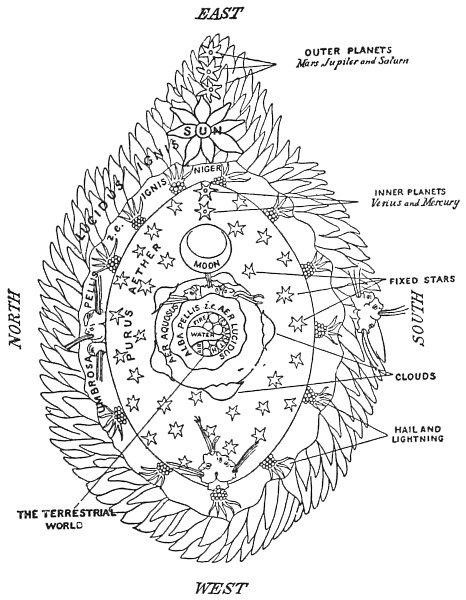
\includegraphics[width=0.5\textwidth]{universe-egg.jpg}
\end{center}
{\tiny{El Huevo Cósmico de Hildegarda von Bingen (1098-1179). Aparece en su obra "Scivias" y es una de las ilustraciones cosmológicas más notables de la Edad Media. Es una representación visual de su visión del universo que combina elementos teológicos cristianos con conceptos cosmológicos.}}


\end{titlingpage}

\endgroup

% As the zine is so short, you probably won't need page numbers; however, if you
% want them, comment out the next line with a %.
\pagestyle{empty}


%% CONTENT GOES BELOW


\section{Paso 0: Universos}

La cosmología estudia el orden que le damos al universo. Aquí vamos a expandir este concepto: un universo es cualquier contexto donde podemos observar, interpretar y actuar. Todos vivimos en múltiples universos simultáneamente.

Luego de la meditación guiada, en esta página del cuadernillo, hagan una lista rápida de todos los universos en los que habitan ahora mismo. No piensen demasiado, dejen que las palabras fluyan.

\newpage
\section{Paso 1: Mi lugar en el universo que transformaré}

De todos los universos que listaste, ¿cuál es el que más te gustaría transformar en este momento de tu vida? ¿Por qué?
Márcalo con un círculo y tómate un momento para escribir tu por qué.

Ahora, en este cuadernillo: dibuja el mapa de tu universo elegido, marca tu ubicación actual en él, identifica y nombra los elementos principales. El mapa puede ser abstracto o simbólico. Puedes usar palabras o símbolos. 
\newpage
\section{Paso 2: La mirada profunda}

Ya ubicados en nuestro universo, es momento de observar. Pero no con una mirada superficial, sino con una que se atreve a ver tanto lo visible como lo invisible. Como en la física moderna, que tuvo que aceptar la existencia de la materia oscura y la energía oscura aunque no pudiera verlas directamente.

Responde en este espacio:

1. ¿Qué elementos son visibles a primera vista en este universo?
\vspace{4cm}

2. ¿Qué elementos están ocultos pero sabes que existen?
\vspace{4cm}

3. ¿Qué aspectos te cuesta trabajo observar?
\vspace{4cm}

\newpage

\section{Paso 3: El propósito del universo}

A diferencia de la cosmología física, donde los eventos simplemente suceden sin necesidad de propósito, los universos humanos están llenos de intenciones y significados. Como seres conscientes, constantemente buscamos y creamos sentido.

En cada universo que habitamos hay un origen y un destino, un "de dónde viene todo esto" y un "hacia dónde va". Es momento de explorar el sentido de este universo que has elegido transformar.

Por favor, responde:

1. Sobre el origen:
¿Por qué y por quién existe este universo que estás explorando?  ¿Qué motivó su origen?
\vspace{5cm}

2. Sobre el propósito:
¿Para qué y para quién existe este universo? ¿Qué propósito tiene su evolución?
\vspace{5cm}


\newpage
\section{Paso 4: Las leyes del universo}
Todo universo está en constante cambio. Existe un devenir que conecta el pasado con el futuro.  Este devenir no es caótico: está gobernado por leyes que determinan cómo se transforma todo. En la física, estas leyes son inmutables y universales. En nuestros universos personales, también existen leyes que gobiernan la evolución entre el origen y el propósito que identificaste.

Para descubrir estas leyes, vamos a usar la matriz de la realidad. 

\begin{center}
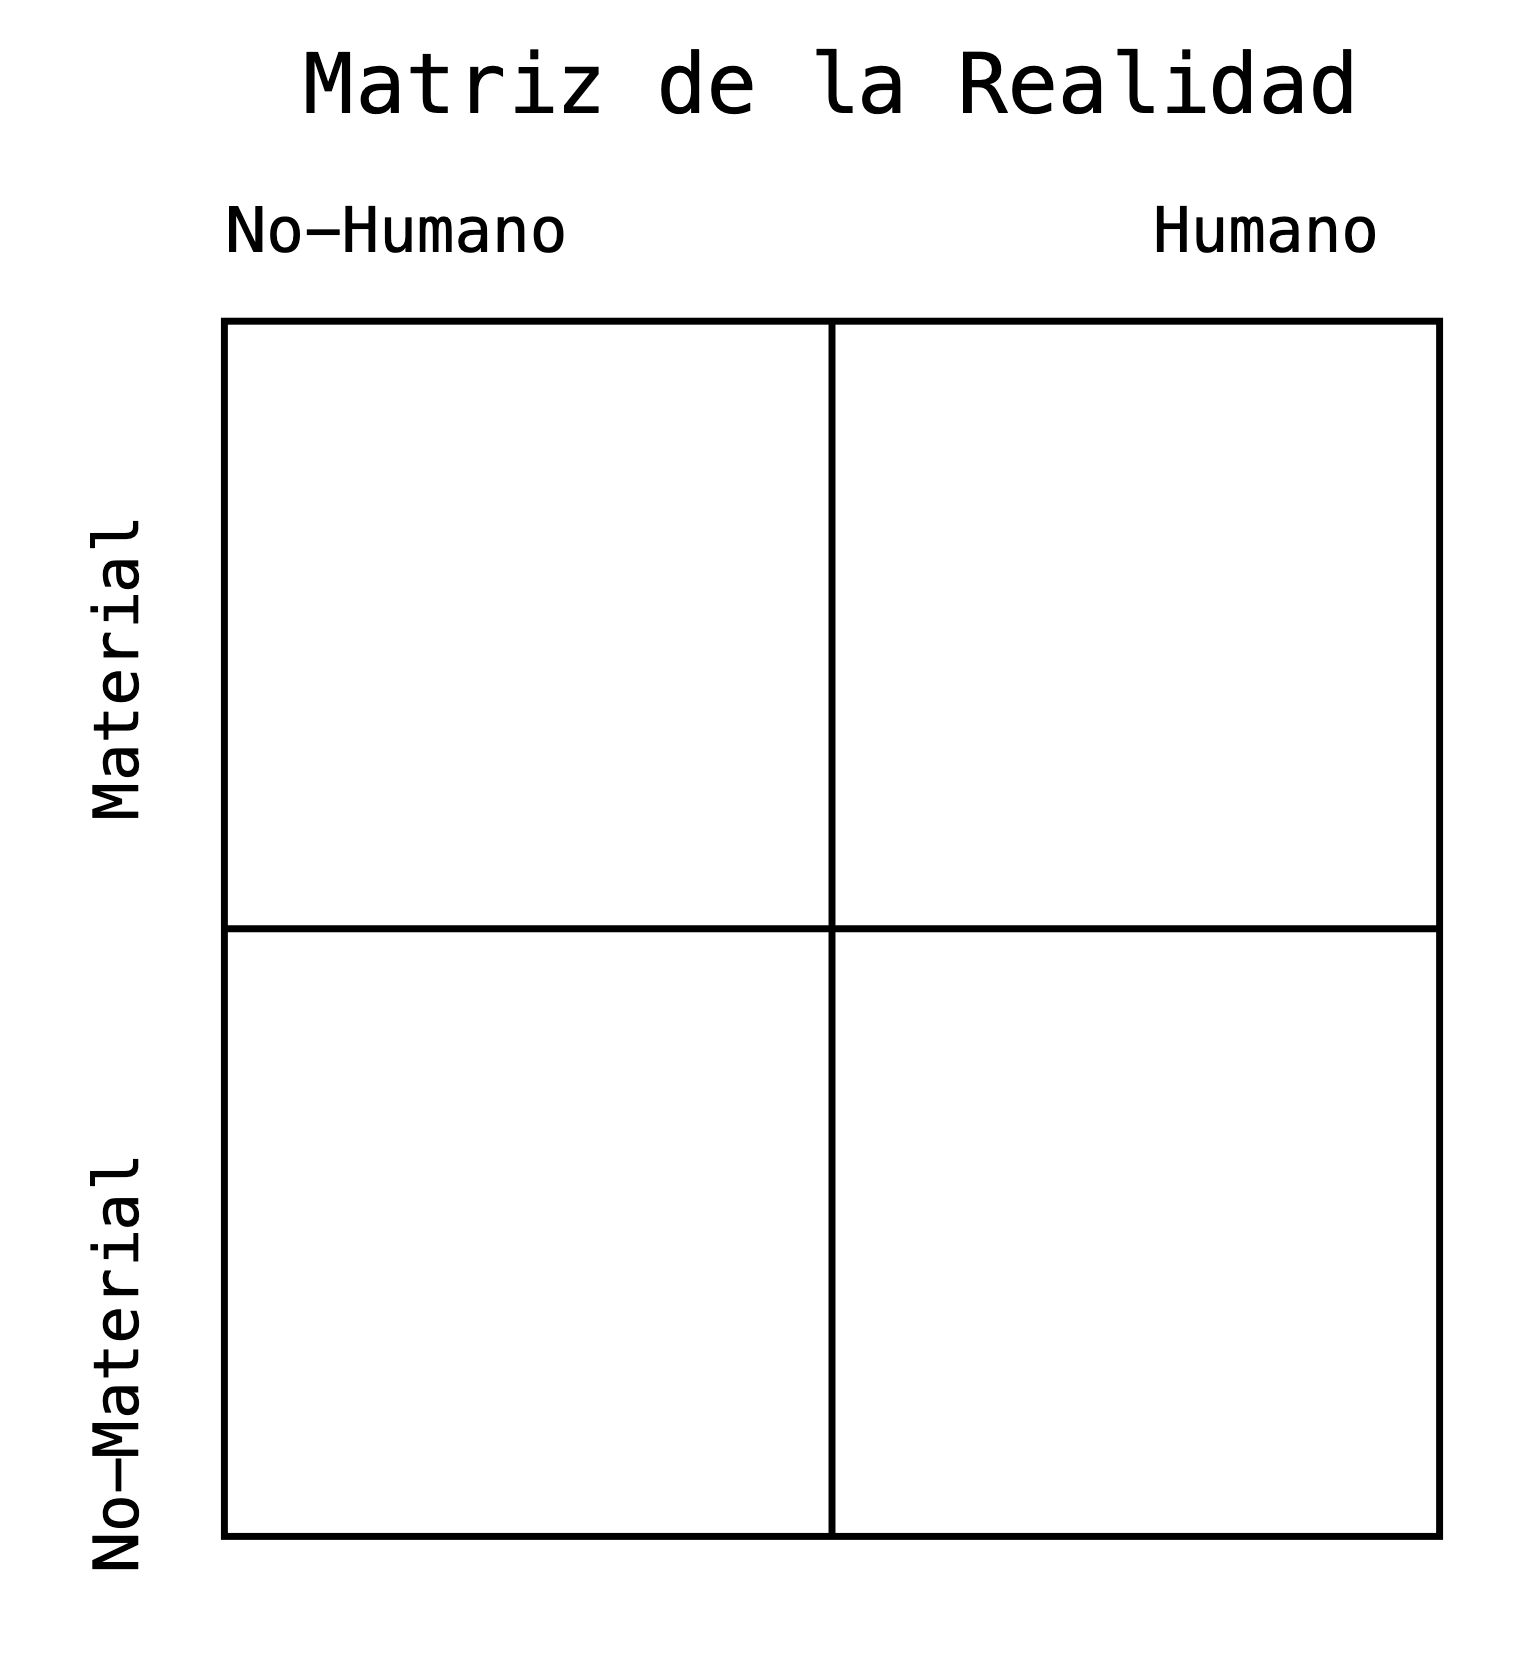
\includegraphics[width=0.7\textwidth]{matriz.png}
\end{center}

Después de completar la matriz, las leyes de tu universo se deberían ubicar en el cuadrante no-humano/no-material.
Ahora, piensa sobre lo siguiente: ¿Qué consecuencias tiene ignorar estas leyes? ¿Cómo puedes usar estas leyes a tu favor?
\vspace{2.5cm}


\newpage
\section{Paso 5: Los elementos del universo}
Las leyes que identificaste gobiernan el comportamiento de elementos concretos, creando patrones de acumulación y dispersión, así como la gravedad gobierna el flujo de la materia en las grandes escalas del Universo.

En la matriz de la realidad que dibujaste, los elementos principales de tu universo se encuentran en el cuadrante no-humano/material. Son las "cosas" concretas que deben fluir y transformarse para que tu universo evolucione.

Responde las siguientes preguntas:

1. ¿Cuáles son los elementos principales que deben transformarse para que este universo evolucione hacia su propósito?
\vspace{3cm}

2. ¿Qué condiciones son necesarias para que estos elementos logren fluir?
\vspace{3cm}

3. ¿Cuál es la mayor obstrucción que identificas en el flujo de alguno de los elementos?
\vspace{3cm}



%% CONTENT ENDS

% Back cover

\newpage
\section{Paso 6: El compromiso de transformación}
Hemos completado un ciclo cosmológico: observación profunda, interpretación sincera y ahora llegamos al momento de la acción concreta. Este movimiento triple refleja tanto el método científico como antiguas prácticas de sabiduría.

El objetivo de este paso final es transformar el conocimiento en sabiduría a través de una acción concreta en el mundo.

Por favor, completa el siguiente manifiesto de acción:

\begin{center}
\textbf{Manifiesto de Acción Cosmológica}
\end{center}

En el universo de \\
\rule{\textwidth}{0.1pt}

Me encuentro en \\
\rule{\textwidth}{0.1pt}

Y desde allí observo que \\
\rule{\textwidth}{0.1pt}

Por eso creo que el origen y el propósito de este universo son \\
\rule{\textwidth}{0.1pt}

He observado que los elementos y leyes principales en este universo son \\
\rule{\textwidth}{0.1pt}

Y he identificado un bloqueo en el flujo de\\
\rule{\textwidth}{0.1pt}

\vspace{1cm}
Por lo tanto, para remover ese bloqueo y ayudar a cumplir de la manera más bella, bondadosa y sincera el propósito de este universo, me comprometo a:

\vspace{0.5cm}
Ir a: \rule{8cm}{0.1pt}

El día: \rule{8cm}{0.1pt}

A la hora: \rule{8cm}{0.1pt}

Para: \rule{8cm}{0.1pt}

\vspace{0.1cm}
Firma: \rule{8cm}{0.1pt}

\end{document}
